\chapter{Problem Classification in Review Websites}

% --- INTRODUCTION ---
\section{Introduction}
Software quality and success is strongly affected by its quality-in-use (QU), usability and user experience (UUX) \cite{Bakiu2017}. User reviews on review websites (e.g. SourceForge\footnote{https://sourceforge.net/}) allow users to report issues when using the software. The user reviews contain lots of valuable information regarding the QU and UUX of software. Unfortunately, this information is hard to access and consume as the reviews have varying quality, an unstructured nature, are available in large numbers and are missing grammatical correctness. Tools are needed that automatically analyze user reviews, thus allowing the processing and usage of the information provided in reviews.

In this chapter, two approaches are discussed which allow an automated analysis and classification of user reviews from review websites. The next section describes the literature search. Then, the two approaches are explained including the algorithms, their evaluation and concrete examples. At last, the two approaches are compared before a conclusion is drawn. For terms regarding requirements engineering, natural language processing, machine learning or used tools, please refery to the glossary.


% --- Literature Search ---
\section{Literature Search}
Given the paper \textit{Which feature is Unusable? Detecting Usability and User Experience Issues from User Reviews} by Bakiu et al \cite{Bakiu2017}, the first step is to define a research question. The research question guiding the literature search is
\begin{quote}
    \textit{How can features or issues of software be classified and evaluated based on user reviews from review websites?}
\end{quote}

The literature search is then performed by two techniques, namely (1) snowballing and (2) term-based search. To be able to tell the relevance of different articles relevance criteria is defined:
\begin{enumerate}
    \item The article should describe how software can be evaluated based on user reviews from review websites as this is the topic of the paper by Bakiu et al.
    \item The article should describe an automated approach to classify features[LINK TO GLOSSAR]/issues[LINK TO GLOSSAR] of software because this is the methodology by Bakiu et al.
    \item The article should contain a classification of user reviews with respect to usability/user experience/quality as this is part of the paper by Bakiu et al.
    \item The article should be written in English. Almost all computer science articles are written in English.
    \item The article should be written by other authors because another methodology should be found.
\end{enumerate}

\subsection*{Snowballing}
The platform that gives access to the paper by Bakiu et al is \textit{IEEE}\footnote{https://ieeexplore.ieee.org/}. Additionally, the platform provides an overview of references and citations of the paper.

The paper references 37 other articles (backward snowballing)  with only one article being relevant for the research question: S. Hedegaard and J. G. Simonsen: 2013 - \textit{Extracting usability and user experience information from online user reviews}\cite{Hedegaard2013}. It is cited five times (forward snowballing). These articles turned out to be not relevant.

\subsection*{Term-based search}
For the term-based search \textit{IEEE}, \textit{ACM}\footnote{https://dl.acm.org/}, \textit{Elsevier}\footnote{https://www.sciencedirect.com/} and \textit{Springer}\footnote{https://link.springer.com/} are used as search platforms. The four platforms were chosen because they provide access to a large database of scientific publications as well as books and other forms of media.

The search terms that are used for the search (with minimal variations to cover a broader range) are
\begin{itemize}
    \item classification AND user review AND review website AND user experience
    \item user experience AND user review AND usability AND issues
    \item problem classification AND user review
    \item quality AND software AND evaluation AND user reviews
    \item problem classification AND review website
    \item classification AND review website AND user experience
\end{itemize}

The search was done in November 2021. The documentation of the search is displayed in \autoref{fig:literature_search}.

\begin{figure}
    \centering
    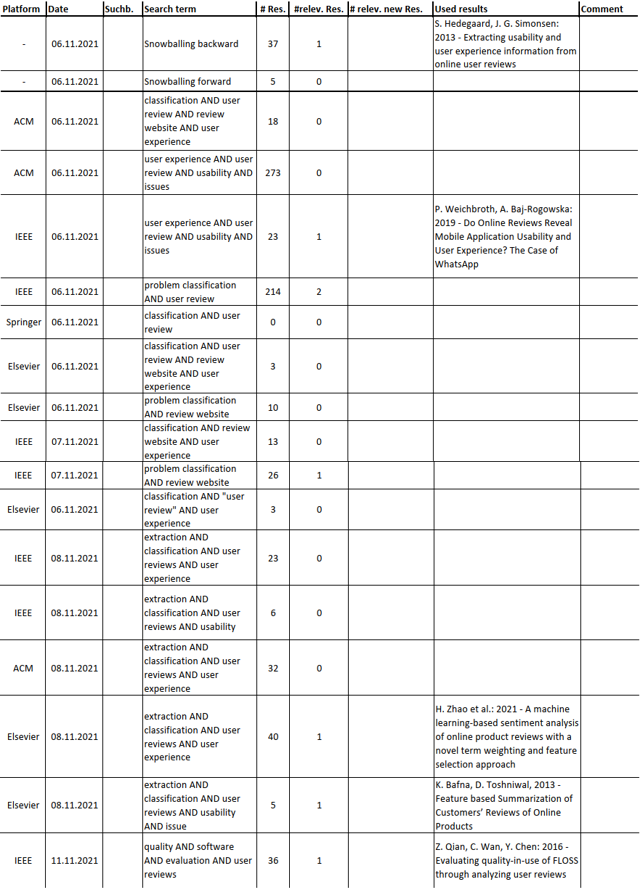
\includegraphics[width=\textwidth]{images/Thema4_LiteratureSearch.png}
    \caption{Literature search documentation}
    \label{fig:literature_search}
\end{figure}

\subsection*{Results}
During the literature search five articles turned out to be of relevance. An overview of the articles with reasons why they are (not) chosen can be found below.

\begin{itemize}
    \item S. Hedegaard, J.G. Simonsen: 2013 - \textit{Extracting usability and user experience information from online user reviews}. The article is not chosen because the article does not describe an automated approach to analyze and classify user reviews with mentioned features.
    \item P. Weichbroth, A. Baj-Rogowska: 2019 - \textit{Do Online Reviews Reveal Mobile Application Usability and User Experience? The Case of WhatsApp}. \cite{Weichbroth2019} The article has a similar topic as the paper by Bakiu et al but is not chosen because the article mainly focuses on mobile app reviews rather than software reviews.
    \item H. Zhao et al: 2021 - \textit{A machine learning-based sentiment analysis of online product reviews with novel term weighting and feature selection approach}. \cite{Zhao2021} The article has a similar topic as the paper by Bakiu et al but is not chosen because the article mainly focuses on products from e-commerce websites rather than software.
    \item K. Bafna, D. Toshniwal: 2013 - \textit{Feature based Summarization of Customers' Reviews of Online Products}. \cite{Bafna2013} The article has a similar topic as the paper by Bakiu et al but is not chosen because the article mainly focuses on products from e-commerce websites rather than software and the classification into usability/user experience/quality topics is missing.
    \item Z. Qian, C. Wan, Y. Chen: 2016 - \textit{Evaluating quality-in-use of FLOSS through analyzing user reviews} \cite{Qian2016}. The article has a similar topic as the paper by Bakiu et al and is chosen because the article has the same topic as the paper by Bakiu et al but a different methodology. The structure of the approach is very similar, but the steps are done differently making the approach suitable for comparison.
\end{itemize}

% --- 1ST APPROACH ---
\section{Approach: Bakiu et al}
% --- Goal ---
\subsection{Goal}
The approach aims to automatically extract and visualize the level of user satisfaction with the UUX dimensions of specific software features that are expressed via user reviews in review websites.

% --- Algorithm ---
\subsection{Algorithm}
The algorithm consists of five steps that are shown in \autoref{fig:approach1_mainsteps}. First, features mentioned in user reviews are extracted. Next, the sentiment[LINK TO GLOSSAR] of the review sentences is analyzed. Features and sentiment are then mapped. In the third step, machine learning classifiers are used to classify UUX issues related to features mentioned in the reviews. Afterwards, the mined information is aggregated and visualized to make it easily consumable. The different steps are explained in detail below.

\begin{figure}
    \centering
    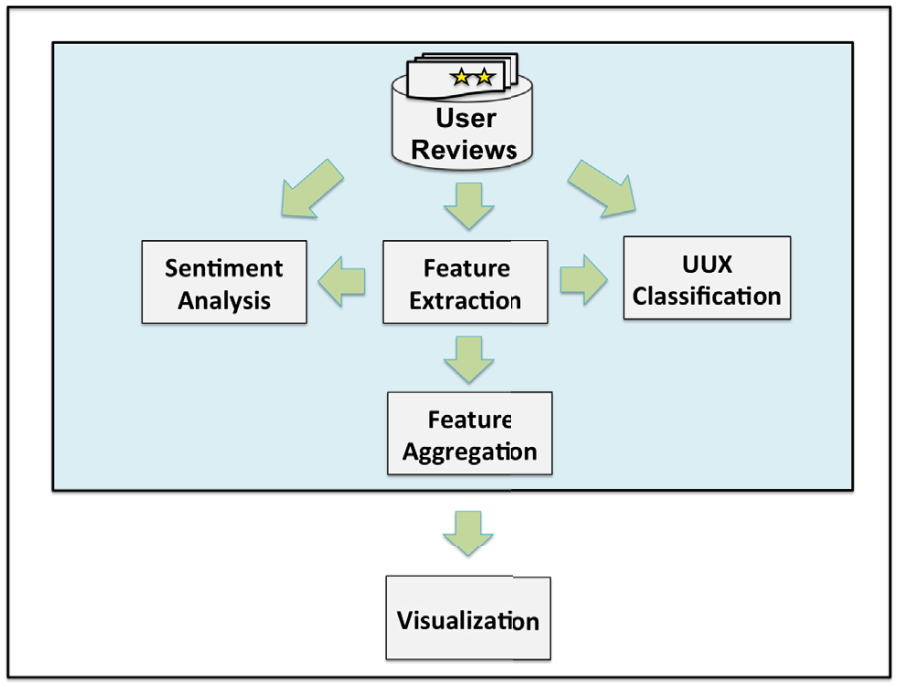
\includegraphics[width=0.7\textwidth]{images/Thema4_Approach1_MainSteps.png}
    \caption{Overview of the main steps of the approach \cite[Figure 1]{Bakiu2017}}
    \label{fig:approach1_mainsteps}
\end{figure}

\subsubsection*{Feature Extraction}
First, the review text is filtered to consider only nouns, verbs and adjectives. These kinds of words are generally used to describe features. To do this, a POS tagger[LINK TO GLOSSAR] of NLTK[LINK TO GLOSSAR] is used. Furthermore, all stop-words[LINK TO GLOSSAR] and common words in user reviews unrelated to software features are removed (e.g. the name of the concerned software, ''please'' and ''fix''). After that, a collocation[LINK TO GLOSSAR] finding algorithm of NLTK is used as features can usually be described through collocations. Word ordering within collocations is ignored for the purpose of extracting feature descriptors. All collocations appearing in less than three reviews and having a distance of less than three words between them are removed. At last, collocations whose pairs of words are synonyms (based on WordNet[LINK TO GLOSSAR] as dictionary) are grouped.

\subsubsection*{Sentiment Analysis}
The sentiment analysis of user reviews is done with the help of SentiStrength[LINK TO GLOSSAR]. The input text is divided into sentences and a positive and negative value is assigned to each sentence. The positive values have a [+1, +5] range, where +5 represents a very positive sentiment. Similarly, the negative sentiments have a range of [-5, -1]. Only words in the reviews that are present in a predefined dictionary are attributed with a sentiment, but modifier words (e.g. ''really''), emoticons and symbols (e.g. ''!'') also alter the sentiment score. The sentiment score of a sentence is calculated by taking the maximum and minimum sentiment scores of all words in the sentence. The sentiment score of a feature is equal to the maximum absolute value of the positive and negative score of the sentence in which it is present. If the absolute positive and negative value is the same, the negative value is assigned to the feature.

This step creates an overview of all extracted features, the frequencies of the features and their sentiment scores.

\subsubsection*{UUX Classification}
In this step, specific UUX information provided in the reviews is detected. The approach uses a taxonomy of UUX dimensions that unify UX dimensions defined by Nielsen (a famous usability consultant) and dimensions from three studies \cite{Bevan2008} \cite{Ketola2008} \cite{BargasAvila2011}. The dimensions are shown in \autoref{tab:uux_dimensions}.

\begin{table} [t]
    \centering
    \begin{small}
    \caption{UUX dimensions of the approach \cite[Table I]{Bakiu2017}}
    \label{tab:uux_dimensions}
    \setlength{\tabcolsep}{1em}
    \begin{tabular}{|l|l|l|l|}
    \hline
    \textbf{Nielsen} & \textbf{Bevan} & \textbf{Ketola} & \textbf{Bargas-Avila} \\
    \hline
    % \hline
    Memorability & Likeability & Anticipation & Affect and Emotion\\
    % \hline
    Learnability & Pleasure & Overall Usability & Enjoyment and Fun\\
    % \hline
    Efficiency & Comfort & Hedonic & Aesthetics and Appeal\\
    % \hline
    Errors/Effectiveness & Trust & Detailed usability & Engagement\\
    % \hline
    Satisfaction & & User Differences & Motivation\\
    % \hline
     & & Support & Enchantment\\
    %  \hline
     & & Impact & Frustration\\
    %  \hline
     & & & Hedonic\\
    \hline
    \end{tabular}
    \end{small}
\end{table}

Supervised machine learning is used to classify described issues into corresponding UUX dimensions. The classification is done on sentence level and one sentence can be associated with multiple UUX dimensions. Therefore, the classification can be seen as a multi-label classification. The approach uses one of the most popular multi-labeling solutions, the binary relevance method (BR) (implementation of scikit-learn[LINK TO GLOSSAR]). BR decomposes the multi-labeling problem into multiple independent binary classification problems. The independent classification results are aggregated to predict the classification of a new instance. The support vector machine[LINK TO GLOSSAR] (implementation of scikit-learn) is used to perform the classification task.

The classifier was trained on a manually labeled collection of reviews from two categories: software (520 reviews) and video games (2972 reviews). Before reviews can be classified, four steps of preprocessing are performed, namely removing stop-words, stemming[LINK TO GLOSSAR] the text, transforming the text into bag of words representation using TF-IDF[LINK TO GLOSSAR] and selecting the best feature according to Chi-Squared metric\footnote{The Chi-Squared metric measures if features are meaningful and have a significant relationship with the response.}. The classifier then assigns UUX dimensions to input sentences. The predicted UUX dimensions are mapped to the features contained in the analyzed sentence.

The output of this step is a list of extracted features and their predicted UUX dimensions.

\subsubsection*{Feature Level Aggregation}
The goal of this step is to aggregate all mined information acquired from the steps before. This is done by averaging the sentiment and unifying the UUX dimensions of all extracted features sharing the same name. This creates a list of features with aggregated sentiment and UUX dimensions.

\subsubsection*{Visualization}
In this step the mined and aggregated information is visualized to ease the consumption. The approach uses the Information Seeking Mantra-method \cite{Shneiderman1996} which states overview first, then zoom and filter and details on demand. Thus, the results of the previous step are visualized in two granularity levels, namely high-level and detailed.

\autoref{fig:approach1_visualization_highlevel} gives a high-level visualization of the results by displaying an overview of the sentiments of UUX dimensions across the most popular features, the rating of reviews over time and the amount of reviews with positive, neutral and negative sentiment.

\begin{figure}
    \centering
    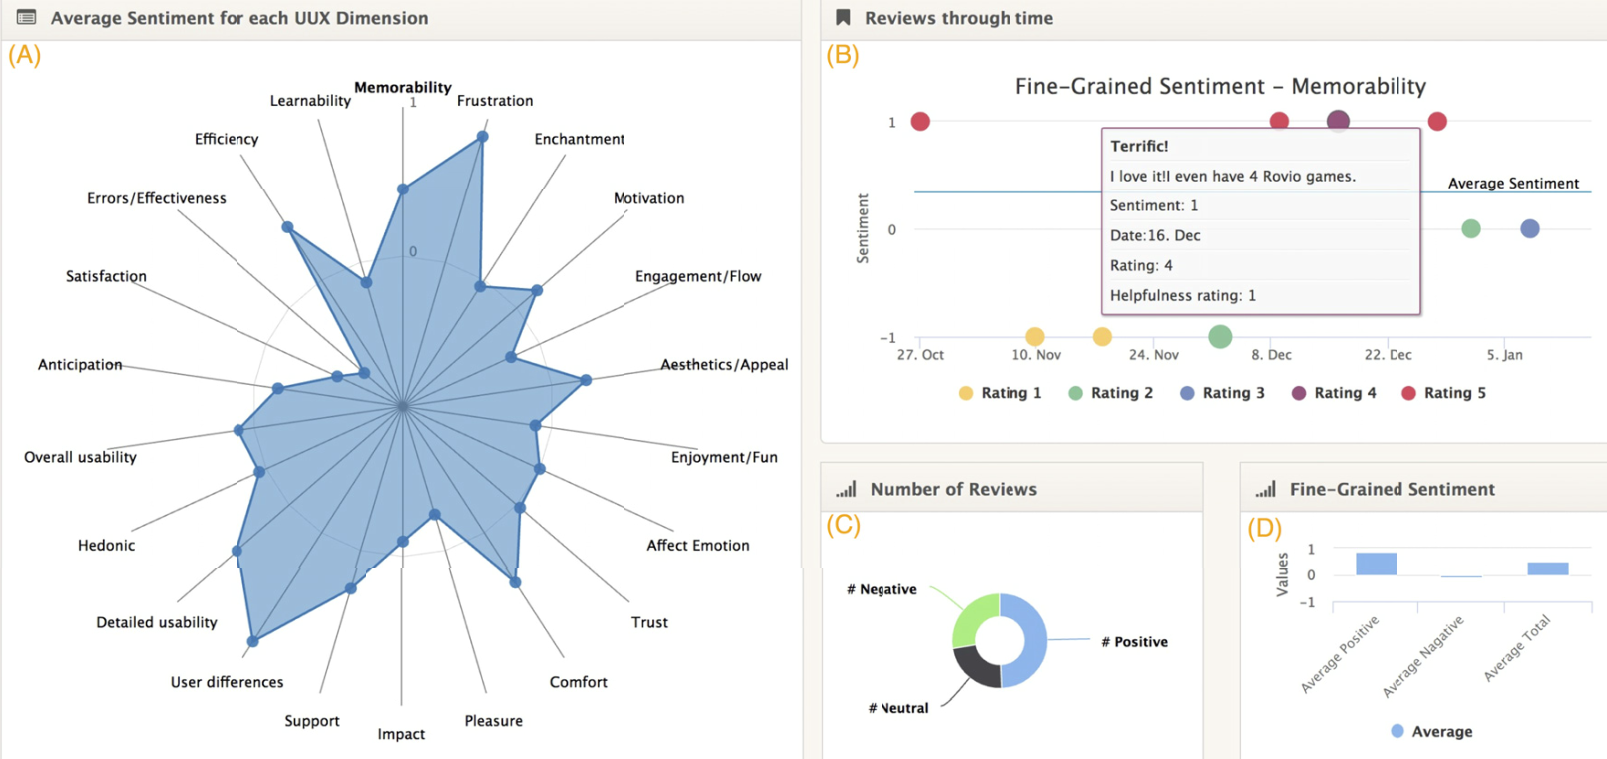
\includegraphics[width=\textwidth]{images/Thema4_Approach1_Visualization_HighLevel.png}
    \caption{High-level visualization of the results \cite[Figure 2]{Bakiu2017}}
    \label{fig:approach1_visualization_highlevel}
\end{figure}

\autoref{fig:approach1_visualization_detailed} provides users with more detailed information about the user acceptance of specific UUX dimensions concerning specific features.

\begin{figure}
    \centering
    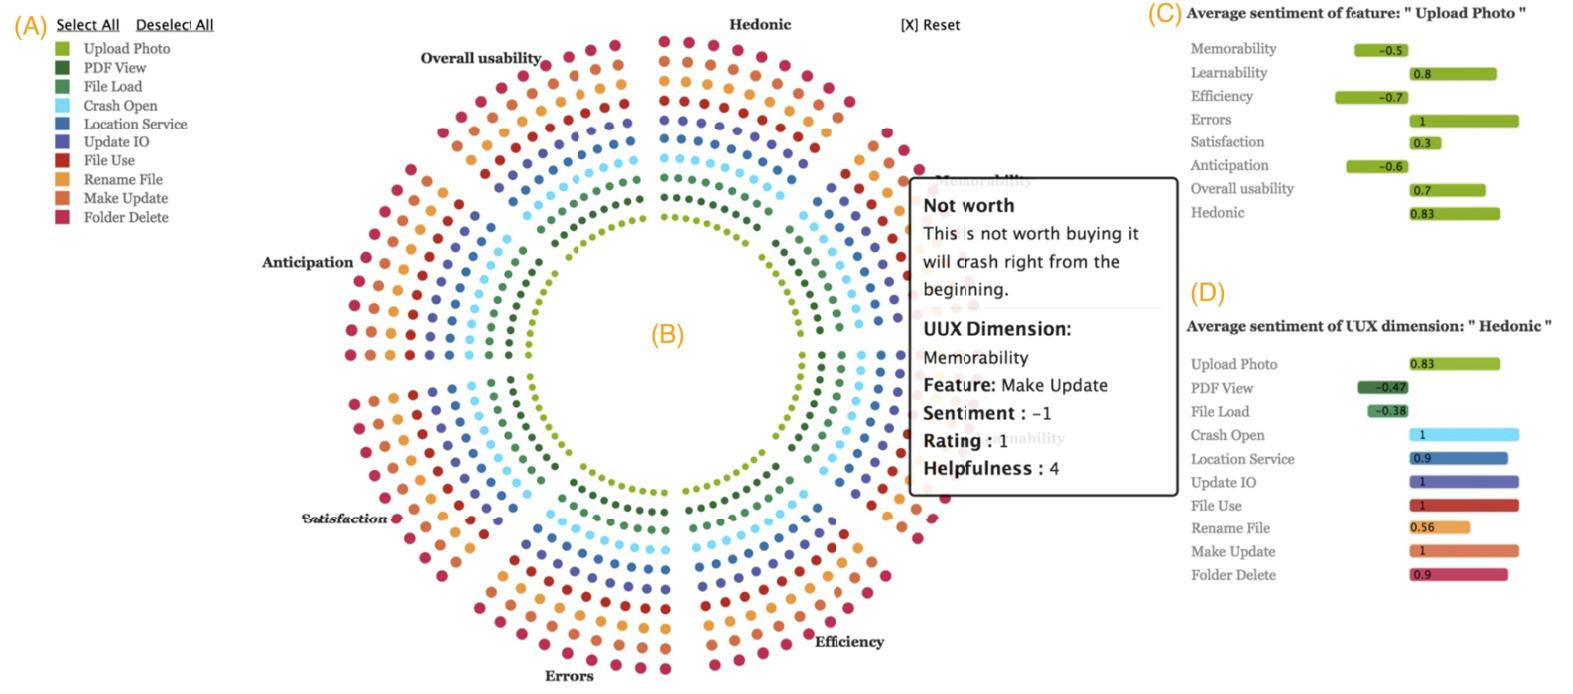
\includegraphics[width=\textwidth]{images/Thema4_Approach1_Visualization_Detailed.png}
    \caption{Detailed visualization of the results \cite[Figure 3]{Bakiu2017}}
    \label{fig:approach1_visualization_detailed}
\end{figure}

% --- Evaluation ---
\subsection{Evaluation}
To evaluate the feasibility and quality of the approach, the approach was run on a collection of user reviews. Then, an opportunistic sampling of 12 correctly extracted and often mentioned features was performed. Only correctly extracted features were considered because the quality of the feature extraction step was already evaluated in a previous work \cite{Guzman2014}. Afterwards, the results produced by the approach were compared with the results of a golden standard (manual sentiment score and UUX dimension assignment). For the comparison, a total amount of 70 sentences were considered.

The common metrics precision[LINK TO GLOSSAR], recall[LINK TO GLOSSAR] and F1-score[LINK TO GLOSSAR] were used to report on the results. The sentiment analysis achieved a precision of 0.68, a recall of 0.64 and a F1-score of 0.64. \autoref{tab:uux_classification_results} shows the UUX classification results at feature level. Dimensions without instances are not included.

\begin{table} [t]
    \centering
    \begin{small}
    \caption{UUX classification results \cite[Table II]{Bakiu2017}}
    \label{tab:uux_classification_results}
    \setlength{\tabcolsep}{1em}
    \begin{tabular}{|l|l|l|l|l|}
    \hline
    \textbf{Dimensions (Frequency)} & \textbf{Precision} & \textbf{Recall} & \textbf{F1-score}\\
    \hline
    Memorability (2) & 1.0 & 0.5 & 0.67\\
    Learnability (5) & 1.0 & 0.4 & 0.57\\
    Errors/Effectiveness (5) & 1.0 & 0.4 & 0.57\\
    Satisfaction (31) & 0.81 & 0.68 & 0.73\\
    Engagement and Flow (16) & 0.9 & 0.53 & 0.67\\
    Detailed Usability (37) & 0.68 & 0.79 & 0.73\\
    Hedonic (7) & 0.8 & 0.5 & 0.62\\
    Pleasure (6) & 0.5 & 0.25 & 0.33\\
    Trust (1) & 0 & 0 & 0\\
    Affect and Emotion (6) & 0.5 & 0.33 & 0.4\\
    Enjoyment, Fun (6) & 0.5 & 0.5 & 0.5\\
    Aesthetics and Appeal (13) & 0.92 & 0.92 & 0.92\\
    Enchantment (1) & 0 & 0 & 0\\
    Frustration (2) & 1.0 & 0.5 & 0.67\\
    \hline
    \textbf{Average} & \textbf{0.69} & \textbf{0.45} & \textbf{0.53}\\
    \hline
    \end{tabular}
    \end{small}
\end{table}

In conclusion, the evaluation shows mixed results. UUX dimensions with a high presence in the test set performed better than dimensions with a low presence. The results are expected to become better with an increasing test set size. The results of the sentiment analysis can be improved by extending the dictionary used in the sentiment analysis step to include software engineering and UUX concepts.

% --- Example ---
\subsection{Example}
Some of the steps are explained using a review containing one sentence:
\begin{quote}
    \textit{Uploading pictures with the app is so terrible!}
\end{quote}

First, the review texts are preprocessed by using a POS tagger to find nouns, verbs and adjectives. Stop-words and a set of words not present in traditional stop-word lists are removed as well. It is assumed that other necessary preprocessing of the text takes place as well although it is not specifically mentioned in the paper by Bakiu et al (e.g. stemming/lemmatization). The example sentence would turn into \textit{upload picture be terrible!}. Next, collocations are found  while ignoring word ordering. Assuming that the collocation \textit{upload picture} occurs in more than two reviews, it is extracted as a feature.

Then, each sentence is assigned two sentiment scores. The example sentence would be assigned the values 1 and -4 based on SentiStrength. Thus, the feature \textit{upload picture} gets a sentiment score of -4 for this sentence.

In the next step, each sentence is assigned a set of UUX dimensions using the trained classifier. The example sentence could be associated with the dimensions \textit{Efficiency} and \textit{Comfort}.

Next, the sentiment scores and UUX dimensions for each feature are aggregated over all reviews. It is assumed that the feature \textit{upload picture} has received the sentiment scores of -2 and -3 and the UUX dimensions \textit{Efficiency} and \textit{Frustration} in sentences of other reviews. An overview can be seen in \autoref{tab:upload_picture}. The aggregated sentiment score for the feature would be -3 (average), the aggregated UUX dimensions \textit{Efficiency}, \textit{Comfort} and \textit{frustration} (union).

\begin{table} [t]
    \centering
    \begin{small}
    \caption{Overview of mined \textit{upload picture} information}
    \label{tab:upload_picture}
    \setlength{\tabcolsep}{1em}
    \begin{tabular}{c|c|l}
    \textbf{Sentence} & \textbf{Sentiment Score} & \textbf{UUX Dimensions} \\
    \hline
    $s_1$ & -4 & Efficiency, Comfort \\
    $s_2$ & -2 & Efficiency \\
    $s_3$ & -3 & Frustration \\
    \end{tabular}
    \end{small}
\end{table}

The results can then be visualized as shown in \autoref{fig:approach1_visualization_highlevel} and \autoref{fig:approach1_visualization_detailed}.

% --- 2ND APPROACH ---
\section{Approach 2: QUIndicator}
% --- Goal ---
\subsection{Goal}
The goal of the approach \textit{QUIndicator} is to evaluate the Quality-in-use of FLOSS (Free/Libre and Open Source Software) based on user reviews from review websites.

% --- Algorithm ---
\subsection{Algorithm}
The algorithm of QUIndicator consists of three main steps that are shown in \autoref{fig:approach2_mainsteps}. First, a topic model is used to cluster user reviews into different topics. The topics are transformed into characteristics (equivalent to \textit{UUX dimensions} from Bakiu et al) of a QU model and the weight of each characteristic is computed. Then, review aspects (equivalent to \textit{features} from Bakiu et al) are taken as the minimum analysis unit and sentiment analysis is applied to analyze the sentiment strength of each review aspect. In the third step, the review aspects are matched to their corresponding characteristics in the QU model and the QU score of the system is evaluated. Wilson Interval[LINK TO GLOSSAR] is used to keep fairness by punishing FLOSS systems with a low amount of reviews. The different steps are explained in detail below.

\begin{figure}
    \centering
    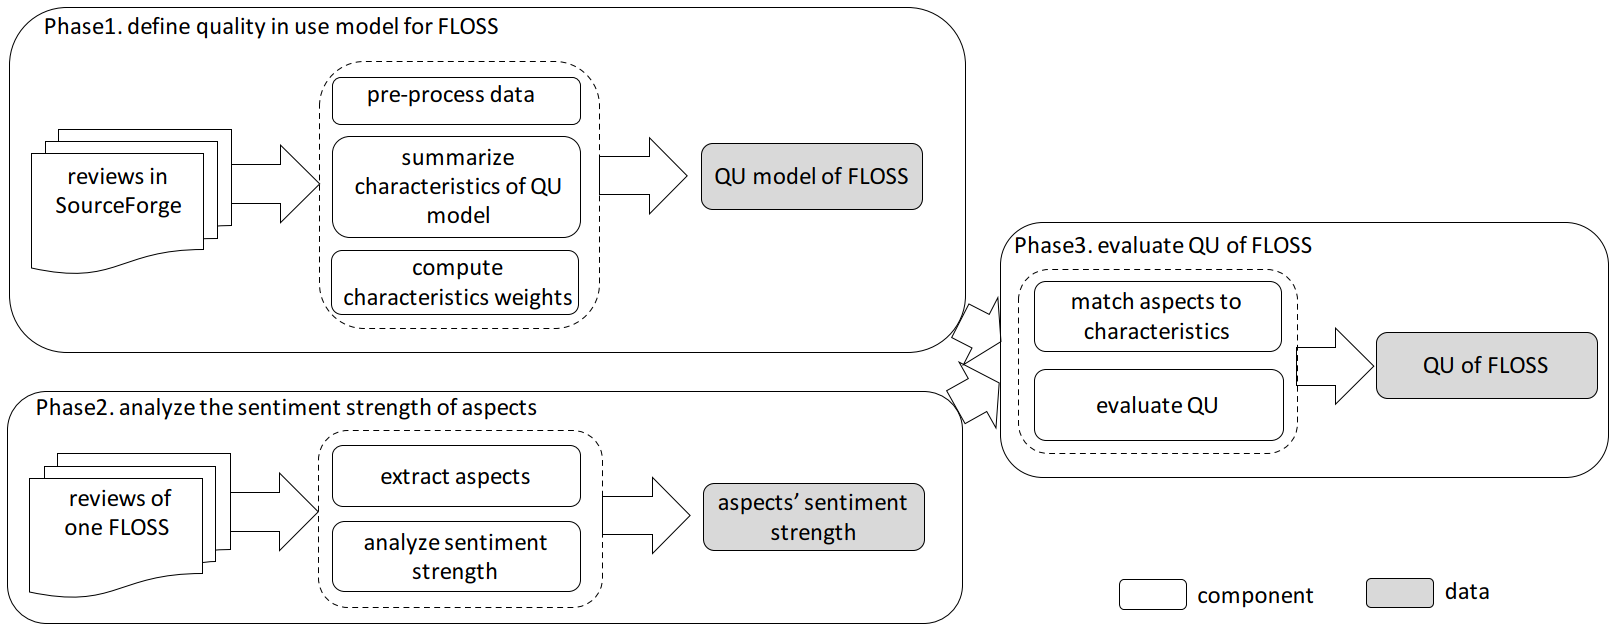
\includegraphics[width=\textwidth]{images/Thema4_Approach2_MainSteps.png}
    \caption{Overview of the main steps of the approach \cite[Figure 1]{Qian2016}}
    \label{fig:approach2_mainsteps}
\end{figure}

\subsection*{Define Quality-in-use Model for FLOSS}

\subsubsection*{Preprocessing data}
Before the reviews can be analyzed, preprocessing of the data takes place. It consists of tokenization[LINK TO GLOSSAR], transformation to lower case, stop-word removal, lemmatization[LINK TO GLOSSAR] and the finding of bigrams. Bigrams[LINK TO GLOSSAR] that appear more than two times are linked by an underscore.

Additionally, the reviews are classified into \textit{informative} and \textit{noninformative} using LingPipe[LINK TO GLOSSAR]. Only informative reviews are considered.

\subsubsection*{Summarizing characteristics of QU model}
To find quality characteristics users may concern, Latent Dirichlet Allocation (LDA)[LINK TO GLOSSAR] is adopted to cluster all user reviews on SourceForge by the date of November 21, 2015. Reviews having implicit semantic relations between them are clustered using 384 topics. The topics can be summarized into five characteristics (with occurring frequency): satisfaction (48.32\%), functionality (22.23\%), safety (12.48\%), usability (8.59\%) and efficiency (8.38\%).

\subsubsection*{Computing characteristic weights}
The characteristic weights can be computed based on the review-topic distribution obtained from LDA. The distribution is shown in \autoref{tab:review_topic_distribution} where $z_k$ represents the \textit{kth} topics and $r_j$ the \textit{jth} review. The weight of a topic can be computed using
\begin{equation}\label{eqn:1}
    Weight(z_k) = \sum_{j=1}^{M} P(z_k|r_j)
\end{equation}
with $z_k$ representing the \textit{kth} topic, $r_j$ the \textit{jth} review and $P(z_k|r_j)$ the probability among the review-topic distribution calculated using LDA. The weight of a characteristic is computed by accumulating the weights of all related topics.

\begin{table} [t]
    \centering
    \begin{small}
    \caption{Review-topic distribution \cite[Table II]{Qian2016}}
    \label{tab:review_topic_distribution}
    \setlength{\tabcolsep}{1em}
    \begin{tabular}{l|l l l l l}
     & $z_1$ & $z_2$ & $z_3$ & ... & $z_K$\\
     \hline
    $r_1$ & 0.302 & 0.000 & 0.004 & ... & 0.209\\
    $r_2$ & 0.001 & 0.020 & 0.204 & ... & 0.007\\
    $r_3$ & 0.320 & 0.000 & 0.004 & ... & 0.331\\
    ... & ... & ... & ... & ... & ...\\
    $r_j$& 0.333 & 0.089 & 0.005 & ... & 0.033\\
    ... & ... & ... & ... & ... & ...\\
    $r_M$ & 0.231 & 0.070 & 0.017 & ... & 0.100\\
    \end{tabular}
    \end{small}
\end{table}

\subsection*{Analyzing Sentiment Strength of Aspects}

\subsubsection*{Extracting aspects}
First, nouns and noun phrases are identified by a POS tagger and their frequencies are counted. Five is set as the threshold, thus nouns/noun phrases occurring more than five times are extracted as aspects. Sentences having infrequent aspects but sentiment words are selected. The noun/noun phrase being closest to the sentiment word is also extracted as an aspect.

\subsubsection*{Analyzing sentiment strength}
A recursive neural tensor network proposed by Socher et al \cite{Socher2013} is adopted and improved to analyze the sentiment strength of aspects. The network is trained by the training set provided by Socher et al\footnote{http://nlp.stanford.edu/sentiment}. The improved version of the network consists of two steps which are shown in \autoref{fig:approach2_network}, namely (1) find all subjects, predicates and objects in a sentence and (2) split them into different parts and find the root node of these parts.

\begin{figure}
    \centering
    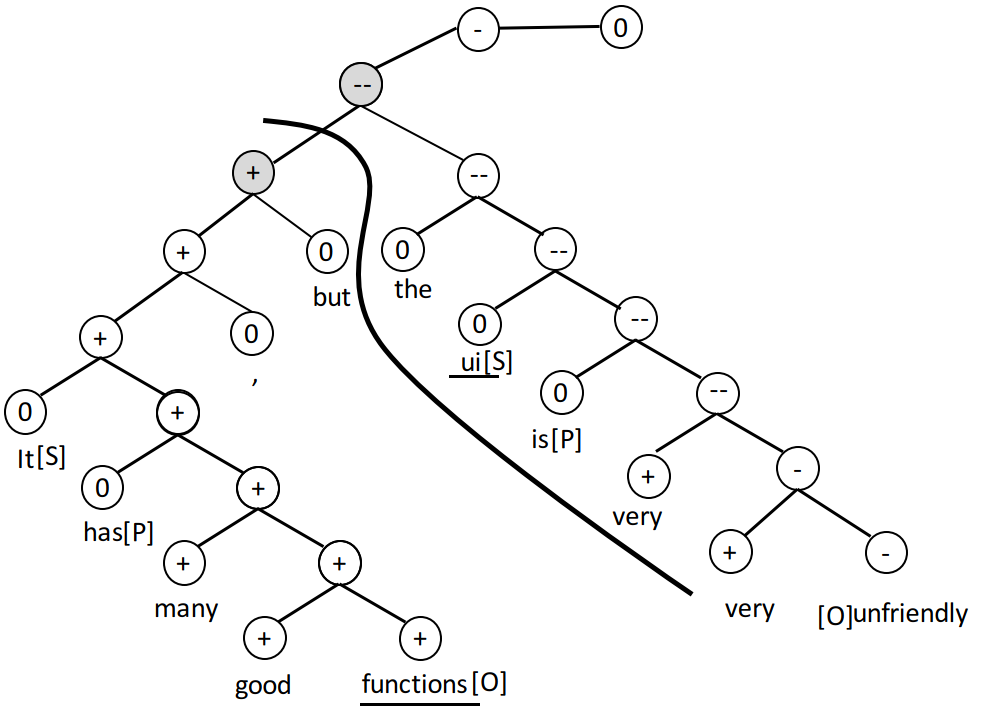
\includegraphics[width=0.75\textwidth]{images/Thema4_Approach2_Network.png}
    \caption{Improved recursive neural tensor network \cite[Figure 2]{Qian2016}}
    \label{fig:approach2_network}
\end{figure}

If one of these parts has an aspect, the score at the root node is its sentiment strength for this review. For the example sentence
\begin{quote}
    \textit{it has many really good functions, but the ui is very very unfriendly}
\end{quote}
shown in \autoref{fig:approach2_network}, the curve splits the sentence into two parts. The gray circles are the root nodes of these parts. The aspect \textit{functions} is assigned a good sentiment strength 4(+), the aspect \textit{ui} is assigned a bad sentiment strength 1(- -). Although it is not explicitly stated in the paper, it can be assumed that the range of sentiment strengths is [- -, + +].

\subsection*{Evaluate QU of FLOSS}

\subsubsection*{Matching aspects to characteristics}
To match extracted aspects to characteristics, Google's Word2Vec[LINK TO GLOSSAR] is used with approx. 190k reviews in SourceForge as training data. Every aspect word is transformed into a word vector of 100 dimensions and a seed word (a word representing the characteristic) is found for every characteristic. The seed word should be in the characteristic and has the smallest cosine similarity with seed words of other characteristics. The different aspects can then be matched to characteristics by calculating their cosine similarity to the seed words. An aspect is matched with a characteristic if the cosine similarity to the seed word is the largest among all characteristics.

\subsubsection*{Evaluating QU}
The last step of the approach consists of computing the QU score of FLOSS. The QU score allows a ranking over different software systems. If a software system has a high QU score and high reputations, it will attract more users and contributors. The proportion of positive rates is balanced with the uncertainty of a small number of observations. Wilson Interval is applied to adjust the confidence degree and punish FLOSS with a low amount of reviews using
\begin{equation}\label{eqn:2}
    WL_{center} = \frac{\hat{p} + \frac{1}{2n}z^2}{1 + \frac{1}{n}z^2}
\end{equation}
where $\hat{p}$ represents the number of positive aspects, $n$ the number of aspects and $z$ the confidence level. For this approach, a confidence level of 95\% is used.

The QU score of FLOSS can then be computed using
\begin{equation}\label{eqn:3}
    QU = \frac{\sum_{j'=1}^{M'} \sum_{s=1}^{S} a_{j', s}W_{C_i}}{M'}WL_{center}
\end{equation}
with $M'$ representing the number of reviews one FLOSS has, $S$ the number of aspects a review has, $a_{j', s}$ the sentiment strength of the \textit{sth} aspect in review $r_{j'}$, $W_{C_i}$ the weight of the \textit{ith} characteristic and $WL_{center}$ the center of Wilson Interval.

% --- Evaluation ---
\subsection{Evaluation}
The approach was evaluated to answer the following research questions:
\begin{enumerate}
    \item What is the accuracy of QUIndicator when it is applied to FLOSS?
    \item How does QUIndicator perform with a low amount of reviews?
\end{enumerate}
To answer the two questions, 30 FLOSS were chosen with a sufficient and a insufficient amount of reviews from ten different genres. Volunteers were asked to read the user reviews and assign QU rank values. To evaluate the accuracy of QUIndicator, two indicators/metrics were applied:

\textbf{Precision@k}
\begin{equation*}
    P@k = \frac{|A \cap K|}{|K|}
\end{equation*}
with $A$ representing the set of the top $K$ FLOSS in the QU rank calculated, $K$ the set of the top $K$ FLOSS in the ground truth, $|A \cap K|$ the number of FLOSS in the set $A$ and the set $K$ at the same time and $|K|$ the number of FLOSS in the set $K$.

\textbf{Spearman Coefficient}
\begin{equation*}
    \rho = 1 - \frac{6 \sum_{i=1}^{N} (s_{1, i} - s_{2, i})^2 }{N(N^2 - 1)}
\end{equation*}
where $s_{1, i}$ represents the \textit{ith} position in QU rank 1, $s_{2, i}$ the \textit{ith} position in QU rank 2 and $N$ the number of positions both QU ranks have. The Spearman Coefficient is between -1 and 1. A value of 1 means the rankings are identical.

The two metrics were combined with the star rating baseline (number of stars given by users) with and without Wilson Interval normalization.

\subsubsection*{Results}
The results for the first research question are shown in \autoref{fig:approach2_precision} and \autoref{fig:approach2_spearman}. QUIndicator shows good results for both $P@3$ and $P@15$. The star rating baseline has a poor performance since many FLOSS systems have five stars in the ground truth making QU ranking random.

\begin{figure}
    \centering
    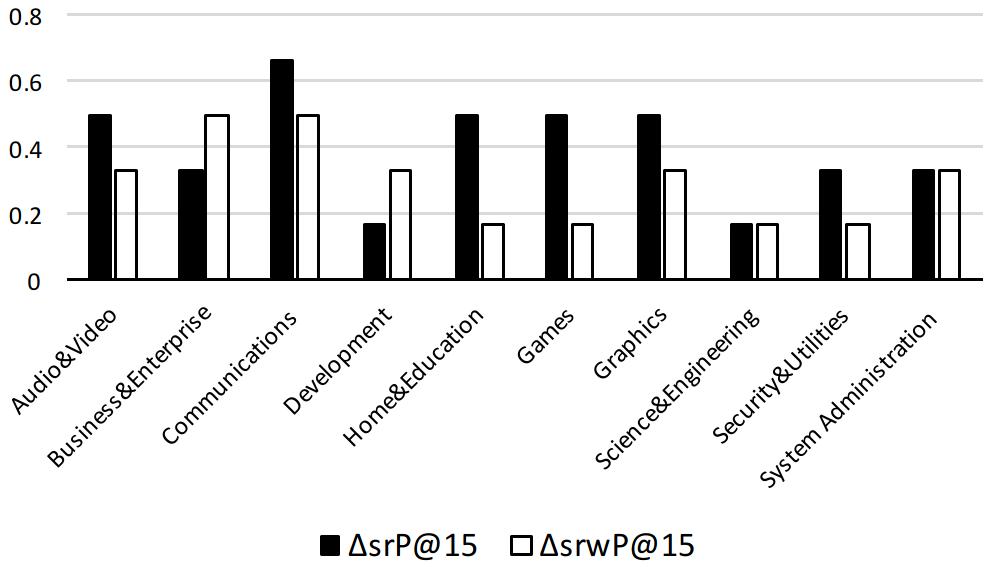
\includegraphics[width=0.7\textwidth]{images/Thema4_Approach2_Precision.png}
    \caption{Results of $P@15$. The horizontal axis represents the FLOSS genre, the vertical axis the precision, $\triangle srP@15$ the precision of $P@15$ minus star rating baseline, $\triangle srwP@15$ the precision minus star rating with Wilson Interval. Based on \cite[Figure 3]{Qian2016}}
    \label{fig:approach2_precision}
\end{figure}

QUIndicator has a high Spearman Coefficient ($>$75\%). This means that the calculated QU ranking is similar to the ground truth.

\begin{figure}
    \centering
    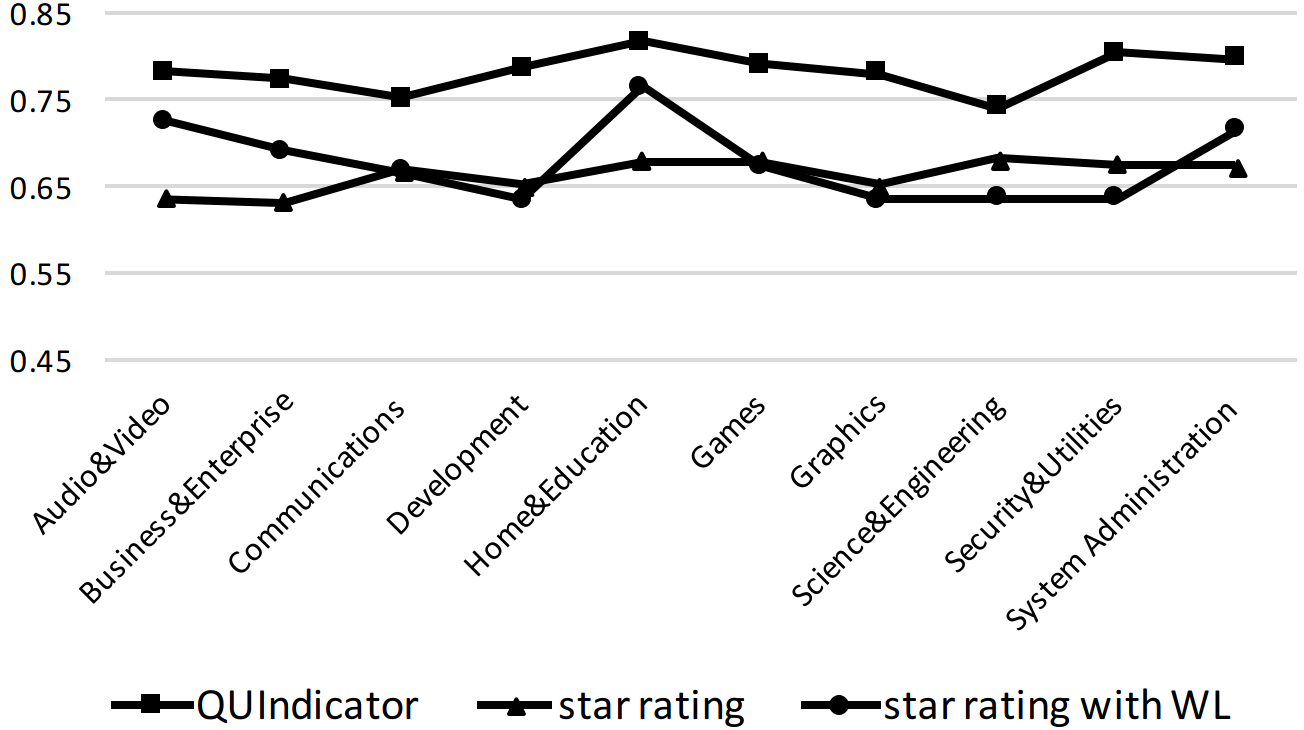
\includegraphics[width=0.7\textwidth]{images/Thema4_Approach2_Spearman.png}
    \caption{Spearman Coefficient of QUIndicator, star rating and star rating with Wilson Interval \cite[Figure 4]{Qian2016}}
    \label{fig:approach2_spearman}
\end{figure}

For FLOSS with a low amount of reviews, $P@3$ and $P@15$ (see \autoref{fig:approach2_precision_insufficient}) showed better results than the star rating baseline which has a poor performance. The Spearman Coefficient is still high but lower than before ($>$55\%).

\begin{figure}
    \centering
    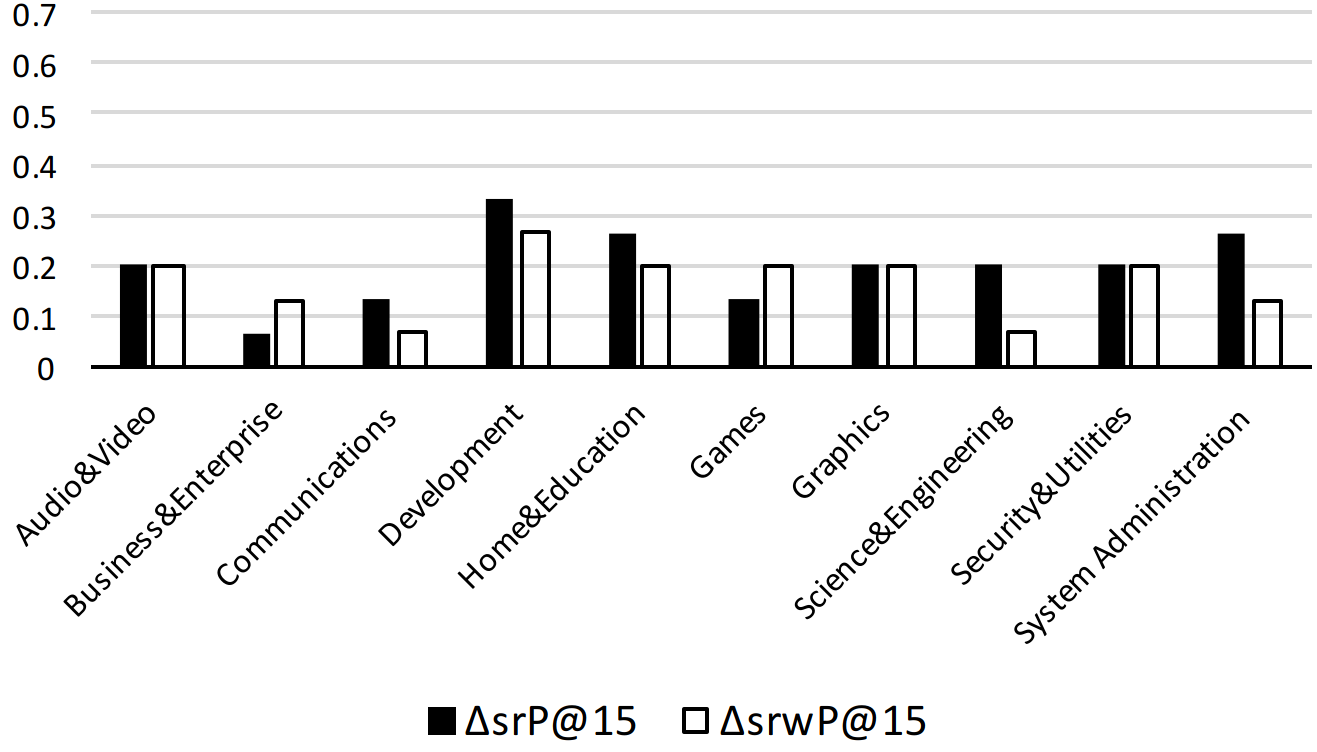
\includegraphics[width=0.7\textwidth]{images/Thema4_Approach2_Precision_Insufficient.png}
    \caption{Results of $P@15$ with a low amount of reviews. The elements in the graph are the same as those in \autoref{fig:approach2_precision}. Based on \cite[Figure 5]{Qian2016}}
    \label{fig:approach2_precision_insufficient}
\end{figure}

% --- Example ---
\subsection{Example}
Some of the steps are explained using a review containing one sentence:
\begin{quote}
    \textit{it has many really good functions, but the ui is very very unfriendly}
\end{quote}

When reviews for a new FLOSS should be analyzed, the first step is to define a QU model used by QUIndicator. It is assumed that the model definition is usually done for multiple FLOSS of the same genre rather than only one FLOSS to make them comparable.

First, LingPipe is used to filter all \textit{informative} reviews. Then, the filtered reviews are preprocessed to define the model. No information about used stop-word lists is provided by Qian et al. Assuming the stop-word list of NLTK, the example sentence would turn into \textit{have good function, ui be unfriendly}. Next, the characteristics are summarized for all reviews using LDA with 384 topics. The result could look like \autoref{tab:summarized_characteristics}. Based on the review-topic distribution, the topics and characteristic weights can then be computed using \autoref{eqn:1}.

\begin{table} [t]
    \centering
    \begin{small}
    \caption{Summarized characteristics, \#topics=384. Based on \cite[Table I]{Qian2016}}
    \label{tab:summarized_characteristics}
    \setlength{\tabcolsep}{1em}
    \begin{tabular}{l|l}
    \textbf{characteristic} & \textbf{frequency (\%)} \\
    \hline
    satisfaction & 48.32\\
    functionality & 22.23\\
    safety & 12.48\\
    usability & 8.59\\
    efficiency & 8.38\\
    \end{tabular}
    \end{small}
\end{table}

Next, aspects are extracted from the reviews. Nouns/noun phrases are tagged by a POS tagger and their frequencies are counted. For the example sentence, \textit{functions} and \textit{ui} would be tagged. Assuming that \textit{functions} and \textit{ui} occur more than five times in the reviews of the FLOSS, they would be extracted as aspects. Then, the sentiment strength of the aspects is determined. The recursive neural tensor network for the example sentence can be seen in \autoref{fig:approach2_network}. The aspect \textit{functions} gets a sentiment score of 4, \textit{ui} a sentiment score of 1.

In the next step, aspects are matched to characteristics. The aspect \textit{functions} could be matched to the characteristic \textit{functionality}, \textit{ui} to \textit{usability}. The center of Wilson Interval is then computed using \autoref{eqn:2}. Finally, the QU score of the FLOSS is calculated using \autoref{eqn:3}. For only this review, the QU score would be calculated by
\begin{equation}
    QU = WL_{center} \sum_{s=1}^{2} a_{s} W_{C_i} = WL_{center} (4 W_{functionality} + 1 W_{usability})
\end{equation}


% --- COMPARISON ---
\section{Comparison}
% --- Summary ---
\subsection{Summary}
The first paper \textit{Which Feature is Unusable? Detecting Usability and User Experience Issues from User Reviews} by Bakiu et al focuses on the analysis of user reviews from review websites with regards to features of software and associated usability and user experience (UUX) dimensions. The approach consists of five steps, namely feature extraction, sentiment analysis, UUX classification, feature level aggregation and visualization. The steps rely on the methods data pre-processing, POS tagger, collocation finding, sentiment analysis with SentiStrength, supervised machine learning and information seeking mantra. The results are visualized using two different kinds of figures. In the end an evaluation of the approach shows mixed results.

The second paper \textit{Evaluating Quality-in-Use of FLOSS through Analyzing User Reviews} by Qian et al describes an approach to evaluate the Quality-in-Use (QU) of FLOSS using user reviews from review websites. The approach can be divided into three major steps, namely QU model definition, sentiment strength analysis of aspects and QU score evaluation. The three steps use the methods data pre-processing, Latent Dirichlet Allocation, POS tagger, sentiment analysis with a recursive neural tensor network and Word2Vec. Additionally, the approach uses Wilson Interval to punish FLOSS with a low amount of reviews, thus keeping fairness among the QU of different FLOSS. After the classification is completed, the approach computes a QU score for each software system based on the extracted information to create a ranking between them. In the end, the evaluation of this approach shows good results for FLOSS having numerous reviews and for FLOSS with a small number of reviews.

% --- Synthesis ---
\subsection{Synthesis}
\subsubsection*{Paper 1}
The approach of the first paper has no specific name associated with it, thus it will be referred to as \textit{Bakiu et al}. The approach can be divided into the following five methods:

\begin{enumerate}
    \item \textbf{Feature extraction:} In this step, features mentioned in user reviews are extracted from the reviews.
    \item \textbf{Sentiment analysis:} During this step, each sentence is assigned a positive and negative sentiment value. The sentiment score of a feature is equal to the maximum absolute score of the sentence in which it is present.
    \item \textbf{UUX classification:} This step uses supervised machine learning to classify sentences into UUX dimensions. The predicted UUX dimensions are assigned to all features extracted from the sentence.
    \item \textbf{Feature level aggregation:} In this step the sentiments are averaged and the UUX dimensions of all extracted features are unified across all reviews.
    \item \textbf{Visualization:} To make the data accessible in an easier way it is visualized with two different granularity levels by applying the Information Seeking Mantra: Overview - Zoom \& Filter - Details on demand.
\end{enumerate}

This approach gives an overview of features and corresponding UUX dimensions by classifying reviews into features and UUX dimensions on sentence level. Additionally, the features/dimensions are mapped to a sentiment score indicating the user's satisfaction with the feature/dimension.

By analyzing the reviews with respect to features and UUX of software developers can find out which functionalities of their software are liked by users, and which are not. This data can be used to drive software development/maintenance efforts when employing software in a particular context making it much easier to address certain issues and to focus on improving them with regards to the UUX dimensions.

The approach was evaluated on a collection of user reviews about video games and software. Features were manually assigned to reviews as well as UUX dimensions associated with them and a sentiment score. The results (manual vs. automated) were compared by computing different measures (precision, recall and F1-score) for the dimensions and the sentiment analysis. The results for the dimensions have an average precision of 0.69, recall of 0.45 and F1-score of 0.53, the results for the sentiment analysis show a precision of 0.68, recall of 0.64 and F1-score of 0.64. The results were mixed regarding the calculated measures (precision, recall and F1-score). Dimensions with a larger presence in the test set achieved better results than other dimensions.

\subsubsection*{Paper 2}
The approach of the second paper by Qian et al is named \textit{QUIndicator} and can be divided into the following three methods:

\begin{enumerate}
    \item \textbf{Defining QU model for FLOSS:} In this step, the QU model is defined by summarizing the reviews into different quality characteristics. Additionally, weights are computed for the characteristics based on their frequency.
    \item \textbf{Analyzing sentiment strength of aspects:} In the second step, aspects are extracted from the reviews. After that, each aspect is assigned a sentiment value to capture the user's satisfaction.
    \item \textbf{Evaluate QU of FLOSS:} To evaluate the QU of a FLOSS, it is necessary to first match aspects to characteristics. After that, the QU score can be computed based on the mined information and Wilson Interval.
\end{enumerate}

This approach gives an overview of aspects and corresponding characteristics by classifying reviews into aspects and characteristics. Additionally, the aspects/characteristics are mapped to a sentiment score indicating the user's satisfaction. Based on this information a QU score is computed.

The QU score gives an overview over different software systems supporting the development and maintenance process. If a software system has a high QU score and high reputations, it will attract more users and contributors to improve the software making developers and users to stakeholders supported by QUIndicator.

The approach was evaluated in two ways. First, it was checked how QUIndicator performs for software with numerous reviews. For this purpose, a value (Precision@K) was defined that provides information about the performance. In addition, the star rating was evaluated, both with and without the Wilson Interval. It turns out that QUIndicator has a good performance for both P@3 and P@15. The star rating baseline has poor performance and the star rating with Wilson Interval baseline also has poor performance. Additionally, the evaluation of the approach is done using the Spearman Coefficient. It turns out that QUIndicator has a high coefficient and is very similar to the ground truth. The second evaluation is for software with few reviews. Here, too, QUIndicator has a good performance for P@3 and P@15. The star rating with and without the Wilson Interval shows poor performance. The Spearman Coefficient is high too ($>$55\%).

% --- Synthesis Matrix ---
\subsection{Synthesis Matrix}
Table \ref{tab:synthesisMatrix} shows the synthesis matrix.

\begin{table}[t]
    \centering
    \begin{small}
    \caption{Synthesis Matrix}
    \label{tab:synthesisMatrix}
    \setlength{\tabcolsep}{1em}
    \begin{tabular}{ p{0.1\textwidth} | p{3cm} | p{4cm} | p{4cm} }
    \hline
    \textbf{Nr.} & \textbf{Name} & \textbf{P1} & \textbf{QUIndicator}\\
    \hline
    \hline
    3a) & Used Methods & data pre-processing, POS tagger, collocation finding, sentiment analysis with SentiStrength, supervised machine learning, information seeking mantra & data pre-processing, Latent Dirichlet Allocation, POS tagger, sentiment analysis with a recursive neural tensor network, Word2Vec\\
    \hline
    3b) & Classification Goal & Features to UUX dimensions, sentiment for each feature & Aspects to characteristics, sentiment strength for each aspect\\
    \hline
    3c) & Data requirements and limitations & - & - \\
    \hline
    4a) & Supported Development Processes & Development, Maintenance & Development, Maintenance\\    \hline
    4b) & Supported Stakeholders & Developer & Developer, User\\
    \hline
    5a) & Tool support / Prototypes & - & QUIndicator \\
    \hline
    5b) & Degree Of Automation & Fully automated & Fully automated \\
    \hline
    6a) & Evaluation & User Review classification was done manually. The results were compared to the calculated results. & User Review classification was done manually. The results were compared to the calculated results of QUIndicator. \\
    \hline
    6b) & Evaluationresults & The results were mixed regarding precision (0.69), recall (0.45) and F1-score(0.53) but can be improved e.g. by extending the used dictionaries. Dimensions with a larger presence in the test set achieved better results than other dimensions. & QUIndicator performs well even with insufficient reviews. $P@3$, $P@15$ and the Spearman Coefficient ($>$55\%) showed better results than the star rating baseline. \\
    \hline
    \end{tabular}
    \end{small}
\end{table}

% --- Differences & Similarities ---
\subsection{Differences \& Similarities}
Both papers describe an approach to analyze and classify software user reviews from review websites. Functionalities of the software are extracted from user reviews and mapped to either UUX dimensions (Bakiu et al) or characteristics (QUIndicator). The two papers use different methods for the extraction of functionalities, UUX dimensions/characteristics and the mapping but have a similar goal.

The extracted functionalities are supplied with a sentiment score in both approaches. The sentiment scores are computed in different ways, either with SentiStrength or by using a recursive neural tensor network.

The first approach visualizes the result allowing an easier consumption of the data. QUIndicator does not visualize the data.

QUIndicator computes a QU score based on the classification and the sentiment analysis to create a ranking between different software. This is not done by Bakiu et al.

% --- CONCLUSION ---
\section{Conclusion}
The two articles discuss two approaches how software user reviews from review websites can be analyzed and classified in an automated way. The two approaches allow the analysis and classification independently from the amount of reviews, their structure and grammatical correctness. Thus, the development and maintenance process of software can be improved by considering the information provided via the reviews.

This means a gain for both developers as well as users. On one hand, with the ability of considering reviews it becomes easier to prioritize software issues effectively as it is clear which issues bother users the most. On the other hand, it is more likely that issues reported by users are fixed/changed. Additionally, developers gain a detailed insight on how their software is recognized by users.

With the second approach, users are supported when looking for a specific software as there is a ranking of software from the respective genre.

Both approaches can be improved to achieve better results in the future, but the discussed methodologies lay the foundation with better results than the baseline.
